\documentclass[tikz,crop=true,10pt]{standalone}

\usepackage[sfdefault]{libertine}
\usepackage{sfmath}

\usepackage{tikzlings}
\usepackage{amsbsy}

 
%flatuicolors.com Flat UI
\definecolor{myblue}{RGB}{41, 128, 185}
\definecolor{myviolet}{RGB}{142, 68, 173}
\definecolor{myorange}{RGB}{211, 84, 0}
\definecolor{mylightbeige}{RGB}{248, 239, 186}
\definecolor{mylightblue}{RGB}{130, 204, 221}

\begin{document}

\usetikzlibrary{arrows.meta, calc}
 
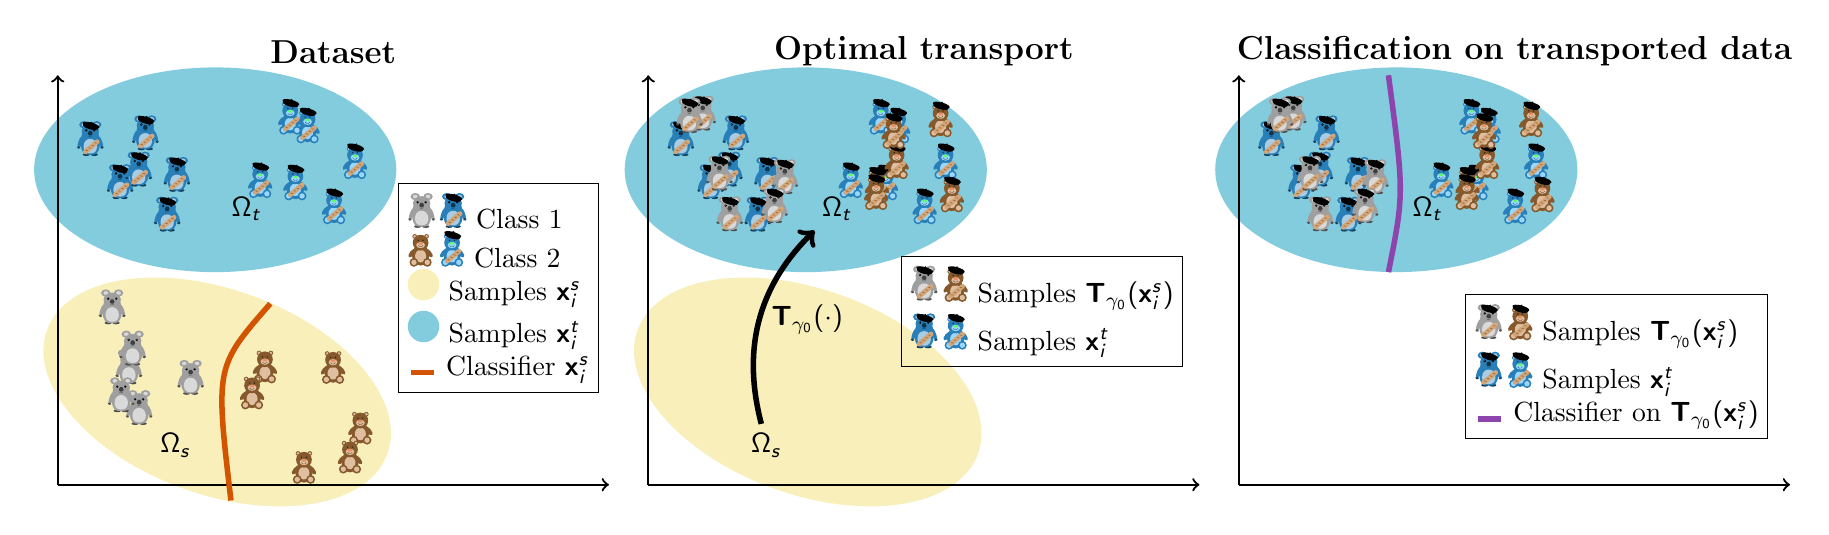
\begin{tikzpicture}

\pgfmathsetseed{3}
\begin{scope}
\fill [mylightbeige, rotate=-20] (1.5,1.8) ellipse (2.3 and 1.3); 
\fill [mylightblue] (2, 4) ellipse (2.3 and 1.3);

\draw[thick,->] (0,0) -- (7,0);
\draw[thick,->] (0,0) -- (0,5.2);

\foreach \x in {1,2,...,6}{
	\pgfmathsetmacro{\mxs}{30+20*rand}
	\pgfmathsetmacro{\mys}{110+20*rand}
	\pgfmathsetmacro{\bxs}{90+20*rand}
	\pgfmathsetmacro{\bys}{110+20*rand}
	\koala[body=myblue,baguette,beret,xshift=\mxs, yshift=\mys,scale=0.2];
	\bear[body=myblue,baguette,beret,xshift=\bxs, yshift=\bys,scale=0.2]}
	
\foreach \x in {1,2,...,6}{
	\koala[xshift=30+20*rand, yshift=40+20*rand,scale=0.2];
	\bear[xshift=90+20*rand, yshift=20+20*rand,scale=0.2]}

\draw[line width=2, myorange] (2.2,-0.2)  .. controls (2,1.5) ..  (2.7,2.3);
\node  at (1.5,0.5) {$\Omega_s$};
\node  at (2.4,3.5) {$\Omega_t$};
\node[draw,align=left] at (5.6,2.5) {
\tikz{\koala[scale=0.2];\koala[body=myblue,baguette,beret,xshift=.4cm,scale=0.2]} Class 1\\ 
\tikz{\bear[scale=0.2];\bear[body=myblue,baguette,beret,xshift=.4cm,scale=0.2]}  Class 2\\ 
\tikz{\fill [mylightbeige] (0,0) ellipse (0.2 and 0.2)} Samples $\boldsymbol{x}_i^s$\\
\tikz{\fill [mylightblue] (0,0) ellipse (0.2 and 0.2)} Samples $\boldsymbol{x}_i^t$\\  
\tikz{\draw[line width=2, myorange] (0,0cm) -- (0.3,0cm)} Classifier  $\boldsymbol{x}_i^s$
};
\node at (3.5,5.5) {\bf  \large Dataset};
\end{scope}

\pgfmathsetseed{3}

\begin{scope}[xshift=7.5cm]
\fill [mylightbeige, rotate=-20] (1.5,1.8) ellipse (2.3 and 1.3);
\fill [mylightblue] (2, 4) ellipse (2.3 and 1.3);

\draw[thick,->] (0,0) -- (7,0);
\draw[thick,->] (0,0) -- (0,5.2);

\foreach \x in {1,2,...,6}{
	\pgfmathsetmacro{\mxs}{30+20*rand}
	\pgfmathsetmacro{\mys}{110+20*rand}
	\pgfmathsetmacro{\bxs}{90+20*rand}
	\pgfmathsetmacro{\bys}{110+20*rand}
	\koala[body=myblue,baguette,beret,xshift=\mxs, yshift=\mys,scale=0.2];
	\bear[body=myblue,baguette,beret,xshift=\bxs, yshift=\bys,scale=0.2]}
	
\foreach \x in {1,2,...,6}{
	\pgfmathsetmacro{\mxs}{30+20*rand}
	\pgfmathsetmacro{\mys}{110+20*rand}
	\pgfmathsetmacro{\bxs}{90+20*rand}
	\pgfmathsetmacro{\bys}{110+20*rand}
	\koala[baguette,beret,xshift=\mxs, yshift=\mys,scale=0.2];
	\bear[baguette,beret,xshift=\bxs, yshift=\bys,scale=0.2]}

\node (source)  at (1.5,0.5) {$\Omega_s$};
\node (target)  at (2.4,3.5) {$\Omega_t$};
\draw[line width=2,->]  (source) to [bend left] node[right]   {$\boldsymbol{T}_{\gamma_0}(\cdot)$} (target);
\node[draw,align=left] at (5,2.2) {
\tikz{\koala[baguette,beret,scale=0.2];\bear[baguette,beret,xshift=.4cm,scale=0.2]} Samples $\boldsymbol{T}_{\gamma_0}(\boldsymbol{x}_i^s)$\\ 
\tikz{\koala[body=myblue,baguette,beret,scale=0.2];\bear[body=myblue,baguette,beret,xshift=.4cm,scale=0.2]}  Samples $\boldsymbol{x}_i^t$
};
\node at (3.5,5.5) {\bf \large Optimal transport};
\end{scope}

\pgfmathsetseed{3}
\begin{scope}[xshift=15cm]
\fill [mylightblue] (2, 4) ellipse (2.3 and 1.3);
\draw[thick,->] (0,0) -- (7,0);
\draw[thick,->] (0,0) -- (0,5.2);

\foreach \x in {1,2,...,6}{
	\pgfmathsetmacro{\mxs}{30+20*rand}
	\pgfmathsetmacro{\mys}{110+20*rand}
	\pgfmathsetmacro{\bxs}{90+20*rand}
	\pgfmathsetmacro{\bys}{110+20*rand}
	\koala[body=myblue,baguette,beret,xshift=\mxs, yshift=\mys,scale=0.2];
	\bear[body=myblue,baguette,beret,xshift=\bxs, yshift=\bys,scale=0.2]}
	
\foreach \x in {1,2,...,6}{
	\pgfmathsetmacro{\mxs}{30+20*rand}
	\pgfmathsetmacro{\mys}{110+20*rand}
	\pgfmathsetmacro{\bxs}{90+20*rand}
	\pgfmathsetmacro{\bys}{110+20*rand}
	\koala[baguette,beret,xshift=\mxs, yshift=\mys,scale=0.2];
	\bear[baguette,beret,xshift=\bxs, yshift=\bys,scale=0.2]}


\draw[line width=2, myviolet] (1.9,2.7)  .. controls (2.1,3.7) .. (1.9,5.2);

\node  at (2.4,3.5) {$\Omega_t$};
\node[draw,align=left] at (4.8,1.5) {
\tikz{\koala[baguette,beret,scale=0.2];\bear[baguette,beret,xshift=.4cm,scale=0.2]} Samples $\boldsymbol{T}_{\gamma_0}(\boldsymbol{x}_i^s)$\\ 
\tikz{\koala[body=myblue,baguette,beret,scale=0.2];\bear[body=myblue,baguette,beret,xshift=.4cm,scale=0.2]}  Samples $\boldsymbol{x}_i^t$\\
\tikz{\draw[line width=2, myviolet] (0,0cm) -- (0.3,0cm)} Classifier  on $\boldsymbol{T}_{\gamma_0}(\boldsymbol{x}_i^s)$
};
\node at (3.5,5.5) {\bf  \large Classification on transported data};
\end{scope}

\end{tikzpicture}




% koala -> bear
% marmot -


\end{document}
